%%%%%%%%%%%%%%%%%%%%%%%%%%%%%%%%%%%%%%%%%%%%%%%%%%%%%%%%%%%%%%%%%%%%%%
\section{\label{sec:Contrib-Install}Contrib Module Installation}
%%%%%%%%%%%%%%%%%%%%%%%%%%%%%%%%%%%%%%%%%%%%%%%%%%%%%%%%%%%%%%%%%%%%%%

This section describes how to install various \Term{contrib modules}
in the Condor system.
Some of these modules are separate, optional pieces, not included in
the main distribution of Condor.
Others are integral parts of Condor taken from the development series
that have certain features users might want to install.
Examples are the new SMP-aware \Condor{startd} and the CondorView
collector.  
Both of these modules come with Condor version 6.1 and
later versions.
However, 
these separate modules may be installed,
maintaining most of the stable release,
while not
switching over to using the
development binaries.

%%%%%%%%%%%%%%%%%%%%%%%%%%%%%%%%%%%%%%%%%%%%%%%%%%%%%%%%%%%%%%%%%%%%%%
\section{\label{sec:HTCondorView-Client-Install}
The HTCondorView Client Contrib Module} 
%%%%%%%%%%%%%%%%%%%%%%%%%%%%%%%%%%%%%%%%%%%%%%%%%%%%%%%%%%%%%%%%%%%%%%
\index{HTCondorView!Client}
\index{contrib module!HTCondorView client}

The HTCondorView Client contrib module is used to automatically generate
World Wide Web pages to display usage statistics of an HTCondor
pool.
Included in the module is a shell script which invokes the \Condor{stats}
command to retrieve pool usage statistics from the HTCondorView server, and
generate HTML pages from the results.  
Also included is a Java applet, which graphically visualizes HTCondor 
usage information.  
Users can interact with the applet to customize the visualization and to
zoom in to a specific time frame.
Figure~\ref{fig:view-screenshot} on page~\pageref{fig:view-screenshot}
is a screen shot of a web page created by HTCondorView.  
%  link gone, and script is not working Dec 2012
%To get a further feel for what pages generated by HTCondorView look like,
%view the statistics for the University of Wisconsin-Madison pool 
%by visiting the URL 
%\URL{http://condor-view.cs.wisc.edu/condor-view-applet}.

\begin{figure}[hbt]
\centering
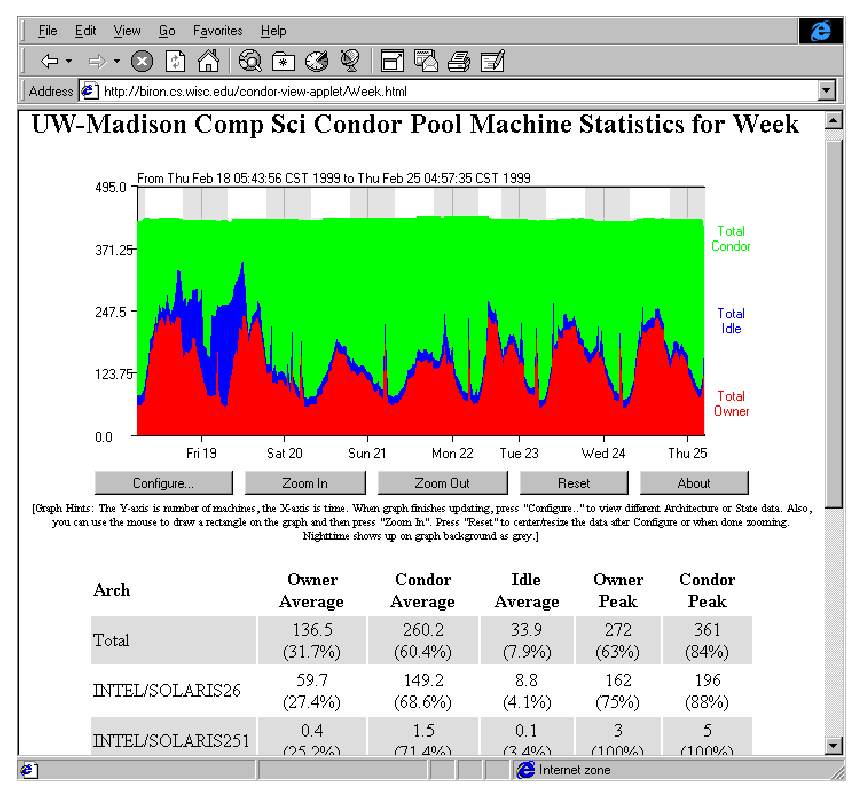
\includegraphics{contrib/view-screenshot.ps}
\caption{\label{fig:view-screenshot}Screen shot of HTCondorView Client}
\end{figure}

After unpacking and installing the HTCondorView Client, a script named
\Prog{make\_stats} can be invoked to create HTML pages displaying HTCondor usage
for the past hour, day, week, or month.  
By using the Unix \Prog{cron} facility to periodically execute
\Prog{make\_stats}, HTCondor pool usage statistics can be kept up to date
automatically.  
This simple model allows the HTCondorView Client to be easily installed;
no Web server CGI interface is needed.

%%%%%%%%%%%%%%%%%%%%%%%%%%%%%%%%%%%%%%%%%%%%%%%%%%%%%%%%%%%%%%%%%%%%%%
\subsection{\label{sec:condorview-client-step-by-step}
Step-by-Step Installation of the HTCondorView Client}
%%%%%%%%%%%%%%%%%%%%%%%%%%%%%%%%%%%%%%%%%%%%%%%%%%%%%%%%%%%%%%%%%%%%%%

\index{installation!HTCondorView Client}
\index{HTCondorView!Client installation}
\begin{enumerate}

\item Make certain that the HTCondorView Server is configured.
Section ~\ref{sec:Contrib-HTCondorView-Install}
describes configuration of the server.
The server logs information on disk in order to provide a persistent,
historical database of pool statistics.
The HTCondorView Client makes queries over the network to this
database.
The \Condor{collector} includes this database support.
To activate the persistent database logging, add the following entries to
the configuration file for the \Condor{collector} chosen to act as the ViewServer.
\begin{verbatim}
    POOL_HISTORY_DIR = /full/path/to/directory/to/store/historical/data 
    KEEP_POOL_HISTORY = True 
\end{verbatim}

\item Create a directory where HTCondorView is to place the HTML files.  
This directory should be one published by a web server, so that HTML
files which exist in this directory can be accessed using a web browser.  
This directory is referred to as the \File{VIEWDIR} directory.

\item Download the \Prog{view\_client} contrib module.
Follow links for contrib modules from the wiki at
\URL{https://htcondor-wiki.cs.wisc.edu/index.cgi/wiki}.

\item Unpack or untar this contrib module into the
directory \File{VIEWDIR}.
This creates several files and subdirectories.
Further unpack the jar file within the \File{VIEWDIR} directory with:
\begin{verbatim} 
  jar -xf condorview.jar
\end{verbatim}

\item Edit the \Prog{make\_stats} script.  At the beginning of the file
are six parameters to customize.
The parameters are

        \begin{description}

	\item[\MacroNI{ORGNAME}] A brief name that identifies an
	organization. An example is ``Univ of Wisconsin''.  Do not
	use any slashes in the name or other special regular-expression
	characters. Avoid the characters \Bs \^\  and \$.

	\item[\MacroNI{CONDORADMIN}] The e-mail
	address of the HTCondor administrator at your site.  
	This e-mail address will appear at the bottom of the web pages.

	\item[\MacroNI{VIEWDIR}] The full path name
	(\emph{not} a relative path) to the \File{VIEWDIR} directory set
	by installation step 2.  
	It is the directory that contains the \Prog{make\_stats} script.

	\item[\MacroNI{STATSDIR}]  The full path name of the
	directory which contains the \Condor{stats} binary.
	The \Condor{stats} program is included in the \Release{bin}
	directory. 
	The value for \MacroNI{STATSDIR} is added to the \MacroNI{PATH}
	parameter by default.  

	\item[\MacroNI{PATH}] A list of subdirectories,
	separated by colons, where the \Prog{make\_stats} script can find
	the \Prog{awk}, \Prog{bc}, \Prog{sed}, \Prog{date}, and \Condor{stats}
	programs.  
	If \Prog{perl} is installed, the path should also
	include the directory where \Prog{perl} is installed.
	The following default works on most systems:
        \begin{verbatim} 
        PATH=/bin:/usr/bin:$STATSDIR:/usr/local/bin
        \end{verbatim}

        \end{description}

\item To create all of the initial HTML files, run
\begin{verbatim}
        ./make_stats setup  
\end{verbatim}
Open the file \File{index.html} to verify that things look good.

\index{HTCondorView!use of \Prog{crontab} program}
\index{crontab program}

\item Add the \Prog{make\_stats} program to \Prog{cron}.  
Running \Prog{make\_stats} in step 6 created a \File{cronentries} file.
This \File{cronentries} file is ready to be processed by the Unix
\Prog{crontab} command.
The \Prog{crontab} manual page contains details about
the \Prog{crontab} command and the \Prog{cron} daemon.
Look at the
\File{cronentries} file; by default, it will run 
\Prog{make\_stats} \Arg{hour} every 15 minutes, 
\Prog{make\_stats} \Arg{day} once an hour, 
\Prog{make\_stats} \Arg{week} twice per day, and 
\Prog{make\_stats} \Arg{month} once per day.
These are reasonable defaults.  
Add these commands to cron on any
system that can access the \MacroNI{VIEWDIR} and
\MacroNI{STATSDIR} directories,
even on a system that does not have HTCondor installed.
The commands do not need to run as root user;
in fact, they should probably not run as root.  These commands can run
as any user that has read/write access to the \File{VIEWDIR} directory.
The command
\begin{verbatim} 
  crontab cronentries
\end{verbatim}
can set the crontab file;
note that this command overwrites the current, existing crontab file with the 
entries from the file \File{cronentries}.

\item Point the web browser at the \File{VIEWDIR} directory
to complete the installation.

\end{enumerate}


%%%%%%%%%%%%%%%%%%%%%%%%%%%%%%%%%%%%%%%%%%%%%%%%%%%%%%%%%%%%%%%%%%%%%%
\section{\label{sec:Ckpt-Server} The Checkpoint Server}
%%%%%%%%%%%%%%%%%%%%%%%%%%%%%%%%%%%%%%%%%%%%%%%%%%%%%%%%%%%%%%%%%%%%%%

\index{installation!checkpoint server}
\index{checkpoint server!installation|(}
\index{HTCondor daemon!condor\_ckpt\_server@\Condor{ckpt\_server}}
\index{daemon!condor\_ckpt\_server@\Condor{ckpt\_server}}
\index{condor\_ckpt\_server daemon}
A Checkpoint Server maintains a repository for checkpoint files.
Within HTCondor, checkpoints may be produced only for standard universe jobs.
Using checkpoint servers reduces the disk requirements of submitting
machines in the pool, since the submitting machines no longer need to
store checkpoint files locally.
Checkpoint server machines should have a large amount of disk space
available, and they should have a fast connection to machines
in the HTCondor pool.

If the spool directories are on a network file system, then
checkpoint files will make two trips over the network: one between the
submitting machine and the execution machine, and a second between the
submitting machine and the network file server.
A checkpoint server configured to use the server's local disk
means that the checkpoint file will travel only once over the
network, between the execution machine and the checkpoint server.
The pool may also obtain checkpointing network performance benefits by
using multiple checkpoint servers, as discussed below.

Note that it is a good idea to pick very stable machines for the checkpoint
servers.
If individual checkpoint servers crash, the HTCondor system will continue to
operate, although poorly.  
While the HTCondor system will recover from a checkpoint server crash
as best it can, there are two problems that can and will occur:
\begin{enumerate}

\item A checkpoint cannot be sent to a checkpoint server that
is not functioning.
Jobs will keep trying to contact the checkpoint server, backing
off exponentially in the time they wait between attempts.
Normally, jobs only have a limited time to checkpoint before they are
kicked off the machine.
So, if the checkpoint server is down for a long period of time,
chances are that a lot of work will be lost by jobs being killed 
without writing a checkpoint. 

\item If a checkpoint is not available from the checkpoint server,
a job cannot be retrieved, and it will either have to be restarted from
the beginning, or the job will wait for the server to come back on line.
This behavior is controlled with the
\Macro{MAX\_DISCARDED\_RUN\_TIME} configuration variable.
This variable represents the maximum amount of CPU time the job is
willing to discard, by starting a job over from its beginning if the
checkpoint server is not responding to requests.

\end{enumerate}

%%%%%%%%%%%%%%%%%%%%%%%%%%%%%%%%%%%%%%%%%%%%%%%%%%%%%%%%%%%%%%%%%%%%%%
\subsection{\label{Prepare-Ckpt-Server} Preparing to Install
a Checkpoint Server} 
%%%%%%%%%%%%%%%%%%%%%%%%%%%%%%%%%%%%%%%%%%%%%%%%%%%%%%%%%%%%%%%%%%%%%%

The location of checkpoint files changes upon the installation
of a checkpoint server.
A configuration change will cause 
currently queued jobs with checkpoints
to not be able to find their checkpoints.
This results in the jobs with checkpoints
remaining indefinitely queued,
due to the lack of finding their checkpoints.
It is therefore best to 
either remove jobs from the queues or let them complete
before installing a checkpoint server.
It is advisable to shut the pool down before doing any
maintenance on the checkpoint server.  
See section~\ref{sec:Pool-Shutdown-and-Restart}
for details on shutting down the pool. 

A graduated installation of the checkpoint server may be
accomplished by 
configuring submit machines as their queues empty.

%%%%%%%%%%%%%%%%%%%%%%%%%%%%%%%%%%%%%%%%%%%%%%%%%%%%%%%%%%%%%%%%%%%%%%
\subsection{\label{Install-Ckpt-Server-Module}
Installing the Checkpoint Server Module} 
%%%%%%%%%%%%%%%%%%%%%%%%%%%%%%%%%%%%%%%%%%%%%%%%%%%%%%%%%%%%%%%%%%%%%%

The files relevant to a checkpoint server are
\begin{verbatim}
        sbin/condor_ckpt_server
        etc/examples/condor_config.local.ckpt.server
\end{verbatim}

\File{\condor{ckpt\_server}} is the checkpoint server binary.
\File{\condor{condor\_config.local.ckpt.server}} is an example
configuration for a checkpoint server. The settings embodied in this
file must be customized with site-specific information.

There are three steps necessary towards running a checkpoint server:
\begin{enumerate}
\item Configure the checkpoint server.
\item Start the checkpoint server.
\item Configure the pool to use the checkpoint server.
\end{enumerate}


\begin{description}

\item[Configure the Checkpoint Server]

\index{checkpoint server!configuration of}
Place settings in the local configuration file of
the checkpoint server.
The file \File{etc/examples/condor\_config.local.ckpt.server} contains
a template for the needed configuration. Insert these into the local
configuration file of the checkpoint server machine. 

The value of \Macro{CKPT\_SERVER\_DIR}  
must be customized.
This variable defines the location of checkpoint files.
It is better if this location is within a very fast local file system,
and preferably a RAID. 
The speed of this file system will have a direct impact on the speed
at which checkpoint files can be retrieved from the remote machines. 

The other optional variables are:
\begin{description}

\item[\Macro{DAEMON\_LIST}] Described in
section~\ref{sec:Master-Config-File-Entries}.  
To have the checkpoint server managed by the \Condor{master},
the \MacroNI{DAEMON\_LIST} variable's value must list both \Expr{MASTER}
and \Expr{CKPT\_SERVER}.
Also add \Expr{STARTD} to allow jobs to run on the checkpoint server machine.
Similarly, add \Expr{SCHEDD} to permit the submission of jobs from the
checkpoint server machine. 

\end{description}

The remainder of these variables are the checkpoint server-specific versions
of the HTCondor logging entries, as described in
section~\ref{sec:Daemon-Logging-Config-File-Entries} on
page~\pageref{sec:Daemon-Logging-Config-File-Entries}.
\begin{description}

\item[\Macro{CKPT\_SERVER\_LOG}] The location of the checkpoint server log.

\item[\Macro{MAX\_CKPT\_SERVER\_LOG}] Sets the maximum
size of the checkpoint server log, before it is saved and the
log file restarted.

\item[\Macro{CKPT\_SERVER\_DEBUG}] Regulates the amount of information
printed in the log file.
Currently, the only debug level supported is \Dflag{ALWAYS}.

\end{description}

\item[Start the Checkpoint Server]

To start the newly configured checkpoint server,
restart HTCondor on that host to enable
the \Condor{master} to notice the new configuration.
Do this by sending a \Condor{restart} command from any machine
with administrator access to the pool.
See section~\ref{sec:Host-Security} on
page~\pageref{sec:Host-Security} for full details about IP/host-based
security in HTCondor. 

Note that when the \Condor{ckpt\_server} starts up, it will immediately
inspect any checkpoint files in the location described by the
\MacroNI{CKPT\_SERVER\_DIR} variable, and determine if any of them are stale.
Stale checkpoint files will be removed.

\item[Configure the Pool to Use the Checkpoint Server]

After the checkpoint server is running,
modify a few configuration variables to let the other machines in the pool
know about the new server:

\begin{description}
   \item[\Macro{USE\_CKPT\_SERVER}] A boolean value that should be set to
   \Expr{True} to enable the use of the checkpoint server.

   \item[\Macro{CKPT\_SERVER\_HOST}] Provides the full host name 
   of the machine that is now running the checkpoint server.  
\end{description}

It is most convenient to set these variables in the pool's
global configuration file,
so that they affect all submission machines.
However, it is permitted to configure each submission machine separately
(using local configuration files), for example if it is desired that not all
submission machines begin using the checkpoint server at one time.
If the variable \MacroNI{USE\_CKPT\_SERVER} is set to \Expr{False},
the submission machine will not use a checkpoint server.

Once these variables are in place,
send the command \Condor{reconfig} to all machines in the pool,
so the changes take effect.
This is described in section~\ref{sec:Reconfigure-Pool} on
page~\pageref{sec:Reconfigure-Pool}.

\end{description}

%%%%%%%%%%%%%%%%%%%%%%%%%%%%%%%%%%%%%%%%%%%%%%%%%%%%%%%%%%%%%%%%%%%%%%
\subsection{\label{Configure-Multiple-Ckpt-Server} 
Configuring the Pool to Use Multiple Checkpoint Servers}
%%%%%%%%%%%%%%%%%%%%%%%%%%%%%%%%%%%%%%%%%%%%%%%%%%%%%%%%%%%%%%%%%%%%%%

\index{checkpoint server!multiple servers}

An HTCondor pool may use multiple checkpoint servers.
The deployment of
checkpoint servers across the
network improves the performance of checkpoint production.
In this case, HTCondor machines are configured to send checkpoints to the
\emph{nearest} checkpoint server.
There are two main performance benefits to deploying multiple checkpoint
servers:
\begin{itemize}
\item Checkpoint-related network traffic is localized by
intelligent placement of checkpoint servers.
\item Better performance implies that jobs spend less time
dealing with checkpoints, and more time doing useful work,
leading to jobs having a higher success rate before returning a
machine to its owner, and workstation
owners see HTCondor jobs leave their machines quicker.
\end{itemize}

With multiple checkpoint servers running in the pool, the
following configuration changes are required to make them active.

Set \Macro{USE\_CKPT\_SERVER} to \Expr{True} (the default) on all
submitting machines where HTCondor jobs should use a checkpoint server.
Additionally, variable \Macro{STARTER\_CHOOSES\_CKPT\_SERVER} should be set to
\Expr{True} (the default) on these submitting machines.
When \Expr{True}, this variable specifies that the checkpoint server
specified by the machine running the job should be used instead of the
checkpoint server specified by the submitting machine.
See section~\ref{sec:Checkpoint-Server-Config-File-Entries} on
page~\pageref{sec:Checkpoint-Server-Config-File-Entries} for more
details.
This allows the job to use the checkpoint server closest to the
machine on which it is running, instead of the server closest to the
submitting machine.
For convenience, set these parameters in the
global configuration file.

Second, set \Macro{CKPT\_SERVER\_HOST} on each machine.
This identifies the full host name of the checkpoint server machine,
and should be the host name of the nearest server to the machine.
In the case of multiple checkpoint servers, set this
in the local configuration file.

Third, send a
\Condor{reconfig} command to all machines in the pool, 
so that the changes take effect.
This is described in section~\ref{sec:Reconfigure-Pool} on
page~\pageref{sec:Reconfigure-Pool}.

After completing these three steps, the jobs in the pool will
send their checkpoints to the nearest checkpoint server.
On restart, a job will remember where its checkpoint was
stored and retrieve it from the appropriate server.
After a job successfully writes a checkpoint to a new server, it will
remove any previous checkpoints left on other servers.

Note that if the configured checkpoint server is unavailable,
the job will keep trying to contact that server.
It will not use alternate checkpoint servers.
This may change in future versions of HTCondor.

%%%%%%%%%%%%%%%%%%%%%%%%%%%%%%%%%%%%%%%%%%%%%%%%%%%%%%%%%%%%%%%%%%%%%%
\subsection{\label{Checkpoint-Server-Domains} 
Checkpoint Server Domains}
%%%%%%%%%%%%%%%%%%%%%%%%%%%%%%%%%%%%%%%%%%%%%%%%%%%%%%%%%%%%%%%%%%%%%%

The configuration described in the previous section ensures that jobs
will always write checkpoints to their nearest checkpoint server.  In
some circumstances, it is also useful to configure HTCondor to localize
checkpoint read transfers, which occur when the job restarts from its
last checkpoint on a new machine.  To localize these transfers, 
it is desired
to schedule the job on a machine which is near the checkpoint
server on which the job's checkpoint is stored.

In terminology, all of the machines configured to use checkpoint
server \Term{A} are in \Term{checkpoint server domain A}.
To localize checkpoint transfers, 
jobs which run on machines in a given
checkpoint server domain should continue running on machines in that domain,
thereby transferring checkpoint files in a single local area of the network.
There are two possible configurations which specify what a
job should do when there are no available machines in its checkpoint
server domain:
\begin{itemize}
\item The job can remain idle until a workstation in its checkpoint
server domain becomes available.
\item The job can try to immediately begin executing on a machine
in another checkpoint server domain.  In this case, the job transfers
to a new checkpoint server domain.
\end{itemize}
These two configurations are described below.

The first step in implementing checkpoint server domains is to include
the name of the nearest checkpoint server in the machine
ClassAd, so this information can be used in job scheduling decisions.
To do this, add the following configuration to each machine:
\begin{verbatim}
  CkptServer = "$(CKPT_SERVER_HOST)"
  STARTD_ATTRS = $(STARTD_ATTRS), CkptServer
\end{verbatim}
For convenience, set these variables in the global configuration file.
Note that this example assumes that
\MacroNI{STARTD\_ATTRS} is previously defined in the configuration.
If not, then use the following configuration instead:
\begin{verbatim}
  CkptServer = "$(CKPT_SERVER_HOST)"
  STARTD_ATTRS = CkptServer
\end{verbatim}
With this configuration, all machine ClassAds will include a \AdAttr{CkptServer}
attribute, which is the name of the checkpoint server closest to this
machine.  So, the \AdAttr{CkptServer} attribute defines the checkpoint
server domain of each machine.

To restrict jobs to one checkpoint server domain,
modify the jobs' \AdAttr{Requirements} expression as follows:
\footnotesize
\begin{verbatim}
  Requirements = ((LastCkptServer == TARGET.CkptServer) || (LastCkptServer =?= UNDEFINED))
\end{verbatim}
\normalsize
This \AdAttr{Requirements} expression uses the \AdAttr{LastCkptServer}
attribute in the job's ClassAd, which specifies where the job last
wrote a checkpoint, and the \AdAttr{CkptServer} attribute in the
machine ClassAd, which specifies the checkpoint server domain.  If the
job has not yet written a checkpoint, the \AdAttr{LastCkptServer}
attribute will be \Expr{Undefined}, and the job will be able to execute in
any checkpoint server domain.  However, once the job performs a
checkpoint,
\AdAttr{LastCkptServer} will be defined and the job will be restricted to the
checkpoint server domain where it started running.

To instead allow jobs to transfer to other checkpoint
server domains when there are no available machines in the current
checkpoint server domain, modify the jobs' \AdAttr{Rank} expression
as follows:
\footnotesize
\begin{verbatim}
  Rank = ((LastCkptServer == TARGET.CkptServer) || (LastCkptServer =?= UNDEFINED))
\end{verbatim}
\normalsize
This \AdAttr{Rank} expression will evaluate to 1 for machines in the
job's checkpoint server domain and 0 for other machines.  So, the job
will prefer to run on machines in its checkpoint server domain, but if
no such machines are available, the job will run in a new checkpoint
server domain.

The checkpoint server domain \AdAttr{Requirements} or \AdAttr{Rank} expressions 
can be automatically appended 
to all standard universe jobs submitted in the pool using
the configuration variables
\MacroNI{APPEND\_REQ\_STANDARD} or \MacroNI{APPEND\_RANK\_STANDARD}.
See section~\ref{sec:Submit-Config-File-Entries} on
page~\pageref{sec:Submit-Config-File-Entries} for more details.
\index{checkpoint server!installation|)}


